\documentclass[a4paper]{exam}

\usepackage{amsmath}
\usepackage{geometry}
\usepackage{tikz}
\usetikzlibrary{backgrounds}

\tikzstyle{arrow} = [->,>=stealth]
\tikzstyle{node} = [auto,font=\footnotesize,draw,circle]

\printanswers

\title{Weekly Challenge 07: Graph Algorithms}
\author{@username}  % replace with your GitHub user names
\date{CS 412 Algorithms: Design and Analysis\\[5pt]Spring 2022}


\begin{document}
\maketitle

\begin{questions}
  
\question
  Consider the graph, $\mathcal{G}$, below with 10 nodes and 13 edges. 
  \begin{center}
    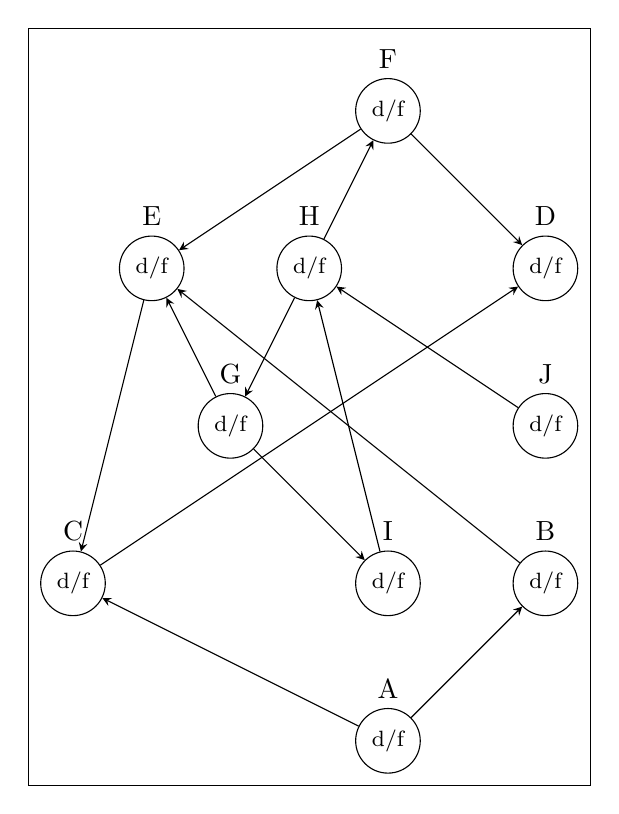
\begin{tikzpicture}[show background rectangle]
      \node[node] [anchor=north, label={A}] (a) at (5, 1) {d/f};
      \node[node] [anchor=north, label={B}] (b) at (7, 3) {d/f};
      \node[node] [anchor=north, label={C}] (c) at (1, 3) {d/f};
      \node[node] [anchor=north, label={D}] (d) at (7, 7) {d/f};
      \node[node] [anchor=north, label={E}] (e) at (2, 7) {d/f};
      \node[node] [anchor=north, label={F}] (f) at (5, 9) {d/f};
      \node[node] [anchor=north, label={G}] (g) at (3, 5) {d/f};
      \node[node] [anchor=north, label={H}] (h) at (4, 7) {d/f};
      \node[node] [anchor=north, label={I}] (i) at (5, 3) {d/f};
      \node[node] [anchor=north, label={J}] (j) at (7, 5) {d/f};

      \draw[arrow] (a) -- (c);
      \draw[arrow] (c) -- (d);
      \draw[arrow] (f) -- (d);
      \draw[arrow] (f) -- (e);
      \draw[arrow] (e) -- (c);
      \draw[arrow] (a) -- (b);
      \draw[arrow] (b) -- (e);
      \draw[arrow] (g) -- (e);
      \draw[arrow] (h) -- (f);
      \draw[arrow] (h) -- (g);
      \draw[arrow] (j) -- (h);
      \draw[arrow] (g) -- (i);
      \draw[arrow] (i) -- (h);
    \end{tikzpicture}
  \end{center}
  The procedure, $\text{DFS}(\mathcal{G})$, is executed on the graph such that ties are resolved in alphabetical order.

  \textbf{TASKS}:
  \begin{parts}
  \part Redraw the graph below such that each node, $n$, contains $n.d/n.f$, where $n.d$ and $n.f$ are the node's discovery and finalization times respectively.
  \part Draw below the corresponding DFS-forest.
  \part Share your drawings in a comment on the \textit{Week 07 Challenge} post in the course group on Yammer.
  \end{parts}
  
  \begin{solution}
    % Enter your solution here.
  \end{solution}
\end{questions}
\end{document}

%%% Local Variables:
%%% mode: latex
%%% TeX-master: t
%%% End:
